\documentclass{book}
\usepackage[utf8]{inputenc}
\usepackage{amssymb}
\usepackage{mathtools}
\usepackage{amsmath}
\usepackage{kotex}
\usepackage{amsthm}
\usepackage{mathrsfs}
\usepackage{footmisc}
\usepackage{enumitem}
\usepackage{stmaryrd}
\usepackage{graphicx}
\usepackage{cutwin}
\usepackage{xypic}
\xyoption{curve}
\usepackage{tikz}
\usepackage{silence}
\DeclareGraphicsExtensions{.pdf,.png,.jpg}
\usepackage[capitalise,nameinlink]{cleveref}
\crefname{prop}{\textbf{Proposition}}{\textbf{Propositions}}
\crefname{thm}{\textbf{Theorem}}{\textbf{Theorems}}
\crefname{lemma}{\textbf{Lemma}}{\textbf{Lemmas}}
\crefname{coro}{\textbf{Corollary}}{\textbf{Corollaries}}
\crefname{ex}{\textbf{Example}}{\textbf{Examples}}
\crefdefaultlabelformat{#2\textbf{#1}#3}

\renewcommand{\thefootnote}{\fnsymbol{footnote}}
\newcommand\dhxrightarrow[2][]{%
  \mathrel{\ooalign{$\xrightarrow[#1\mkern4mu]{#2\mkern4mu}$\cr%
  \hidewidth$\rightarrow\mkern4mu$}}
}

\newtheorem{theorem}{Theorem}[section]
\newtheorem{prop}{Proposition}[section]
\newtheorem{lemma}{Lemma}[section]
\newtheorem{coro}{Corollary}[section]

\theoremstyle{definition}
\newtheorem{defn}{Definition}[section]
\newtheorem{ex}{Example}[section]
\newtheorem*{quest}{Question}
\newtheorem*{remind}{Remind}
\newtheorem*{add}{Additional}


\title{Linear Algebra}
\author{Keonwoo Kim}
\date{\today}

\begin{document}
\tableofcontents{}
\chapter*{Preface}
\addcontentsline{toc}{chapter}{\protect\numberline{}Preface}
This lecture note is based on \textit{Linear Algebra, 2nd edition} by K. Hoffman and R. Kunze.
\chapter{Vector Space}

\section{Matrix}
\begin{remind}
A \textbf{field} is a \textit{good} algebraic structure, which has the addition and the multiplication. Formally, a field $(F,~+,~\cdot)$, or simply $F$, is a pair of a set and two operations which is from $F\times F$ to $F$ satisfying the following:
\begin{itemize}
\item $(F,~ +)$ is an \textbf{abelian group}, that is, $+$ is commutative, associative, and there is an additional identity 0 and the inverse element $-a$ of $a$ for all $a \in F.$
\item $(F^{\times },~\cdot)$ is also an abelian group, that is, $\cdot$ is commutative, associative, and there is an multiplicational identity 1 and the inverse element $a^{-1}$ of $a$ for all $a \in F^{\times},$ where $F^{\times} = F - \{0\}.$
\item + and $\cdot$ are \textit{compatible}, which means $\cdot$ is distributing over $+.$
\end{itemize}
We simply write $a-b := a+(-b)$ and $a/b=ab^{-1}.$

A \textbf{matrix} over a field $F$ is a rectangular arrangement of \textit{scalars}, elements of the field $F$. The space of $m$ by $n$ matrices is denoted as $\mathfrak M_{m,n}(F).$
\end{remind}
\begin{ex}\leavevmode
\begin{itemize}
\item $\mathbb Q$, $\mathbb R$, $\mathbb C$ are well-known(?) fields.
\item $\mathfrak M_{m,n}(F) \approx F^{mn},$ without the product.
\item Matrices do not form a field.
\end{itemize}
\end{ex}

\subsection{Transpose and Trace}
\begin{defn}
For every $m$ by $n$ matrix $A \in \mathfrak M _{m,n}(F),$ the \textbf{transpose} of $A$ is defined as follows: $$ A^{\mathsf T} = (a_{ji})_{n,m}.$$ For every $n$ by $n$ \textit{square} matrix $A \in \mathfrak M_{n,n}(F),$ the \textbf{trace} of $A$ is defined as follows: $$\operatorname{tr}A = \sum_{i=1}^n a_{ii}.$$
\end{defn}

\begin{prop}[Linearity of transpose and trace]
For every pair of $m$ by $n$ matrices $A$ and $B \in \mathfrak M_{m,n}(F)$ and every pair of scalars $a,~b \in F$, $$(aA + bB)^{\mathsf T} = a A^{\mathsf T} + bB^{\mathsf T}.$$ For every pair of $n$ by $n$ square matrices $A$ and $B \in \mathfrak M_{n,n}(F)$ and every pair of scalars $a,~b \in F$, $$\operatorname{tr}(aA + bB) = a \operatorname{tr}A + b \operatorname{tr}B.$$
\end{prop}
\begin{proof}
ㅎㅎ.
\end{proof}

\begin{prop}[Behaviour of transpose and trace]
$$(AB)^\mathsf T = B^\mathsf T A^\mathsf T, \qquad \operatorname{tr}A = \operatorname{tr} A^\mathsf T, \qquad \operatorname{tr}(AB) = \operatorname{tr}(BA).$$
\end{prop}
\begin{proof}
Try it!
\end{proof}


\subsection{Inverse Matrix}
\begin{defn}
For a \textit{square} matrix $A\in\mathfrak M_{n,n}(F),$ if there is another square matrix $B\in\mathfrak M_{n,n}(F)$ such that $$AB = I = BA,$$ then we call $B=A^{-1}$ the(?) \textbf{inverse matrix} of $A$.
\end{defn}

\begin{prop}[Uniqueness of inverse matrix] The inverse matrix of a matrix $A$ is unique (if exists). This justifies the occurrence of \textbf{`the'} above.
\end{prop}
\begin{proof}
Let those be $A^{-1}$ and ${\tilde A }^{-1},$ then $${\tilde A }^{-1} = (A^{-1}A) {\tilde A }^{-1} = A^{-1}(A {\tilde A }^{-1}) = A^{-1}.$$
\end{proof}

\begin{quest} If $AB = I$ for two square matrices $A$ and $B$, what can we say about the invertibility of them? We will solve this problem using a `function,' which is from and to some vector spaces, defined below.
\end{quest}

\newpage

\section{Vector Space}
\begin{defn}
A \textbf{vector space} $V$ over $F$, or simply an \textbf{\textit{F}-vector space} $V$, is a \textit{good} algebraic structure, which has the addition $+:~V\times V \to V$ and the $F$-scalar multiplication $\mathrm{SM}_F:~F\times V \to V$. Formally, a field $(V,~F,~+,~\mathrm{SM}_F)$, or simply $V$, is a pair of a set, a field and two operations satisfying the following:
\begin{itemize}
\item $(V,~ +)$ is an abelian group.
\item $\mathrm{SM}_F$ and $\cdot_F$ are compatible: $(ab)v = a(bv)$ for every $a, ~b \in F$ and $v\in V,$ and $1v = v$ for all $v\in V.$
\item $+$s and $\mathrm{SM}_F$ are compatible: $(a+b)v = av + bv,$ $a(v+w) = av + aw$ for every $a,~b\in F$ and $v,~w \in V.$
\end{itemize}
We simply write $v-w := v+(-w).$
\end{defn}
\begin{ex} The following structures are examples of vector space.
\begin{itemize}
\item \textbf{\{0\}} is a vector space over \textit{arbitrary field}, and is called the \textbf{trivial space.}
\item $\mathbb R^n$ and $\mathbb C^n$ are vector spaces. In fact, for any field $F$, $F^n$ is an $F$-vector space, trivially.
\item Hence, a matrix space $\mathfrak M_{m,n}$ of $m$ by $n$ matrices over $F$ is a vector space since is \textit{the same with} $F^{mn}$, and the polynomial space of $n$-th degree $\mathbf{P}_n [t] = \{\sum_{i=0}^n a_i t^i: ~ a_i \in F\}$ is also a vector space, \textit{the same with} $F^{n+1}.$
\item (Field extension) If there are two fields which one is a subfield of another, namely $E \ge F$, then $E$ is a $F$-vector space, with its addition and multiplication (as a scalar multiplication.)
\item (\textbf{dual space!}) A \textbf{linear functional} $f$ on $V$ is a \textit{linear} map from $V$ to $F$, that is, $$f(av+b) = af(v)+b$$ for every $a,~b\in F$ and $v\in V.$ The \textbf{dual space} of $V$ is the space of linear functionals on $V$, and it forms a $F$-vector space, with the following operations: $$(f+g)(v) = f(v) + g(v),\qquad (af)(v) = af(v).$$ The dual space is one of the most interesting things not only in linear algebra, but in abstract algebra, or even in \textit{any} branches which use the term \textit{dual} (e.g., in projective geometry).
\end{itemize}
\end{ex}


\begin{prop}
\leavevmode

\begin{itemize}

\item $0v = 0$ and $(-1)v = -v$.
\begin{proof} $0v=(0+0)v=0v+0v$ implies $0v=0$ and $v+(-v)=0=0v=(1+(-1))v=1v+(-1)v=v+(-1)v$ implies $-v=(-1)v.$
\end{proof}
\item Every \textbf{linear combination} $\sum_i a_i v_i$ of vectors $v_i \in V$ is in $V.$
\begin{proof} Easy induction on the number of summands(terms).
\end{proof}
\end{itemize}
\end{prop}

\begin{defn}
A subset $W\subseteq V$ is called a \textbf{subspace} of $V$ if it forms a vector space itself with the \textit{inherited} operations from $V$. We denote it $W\le V.$
\end{defn}
\begin{prop}\label[prop]{p:subspace}
$$W\le V~~~\Longleftrightarrow~~~ \forall c\in F,~ \forall v,~w\in W,~~~ cv+w \in W.$$
\end{prop}
\begin{proof}
($\Leftarrow$) The other axioms of vector space is satisfied by the fact that the operations are inherited by $V$, and hence it suffices to show that the operations are closed. First, let $c=-1$ and $v=w.$ Then we have $(-1)w + w = 0 \in W$ by the proposition above. Then, the addition is closed if we let $c=1$; and so is the scalar multiplication if we let $w=0$, which is in $W$, as we proved. Hence $W$ forms a vector space.

($\Rightarrow$) $cv+w$ is a linear combination. ㅋㅋ.
\end{proof}
\begin{ex}
\leavevmode
\begin{itemize}
\item Removing a coordinate(\textbf{projection}): $$F^2 = \left\{(a,b):~a,b\in F\right\} \le \left\{(a,b,c):~a,b,c\in F\right\} = F^3.$$
\item \textbf{Symmetric}, \textbf{alternating} matrices over $F$: $$\mathrm{Sym}_n(F) = \{A \in \mathfrak M_{n,n}(F):~A=A^{\mathsf T}\} \le M_{n,n}(F),$$
$$\mathrm{Alt}_n(F) = \{A \in \mathfrak M_{n,n}(F):~A=-A^{\mathsf T}\} \le M_{n,n}(F).$$
\item \textbf{Hermitian} matrices: $$\mathrm{Her}_n = \{A \in \mathfrak M_{n,n}(\mathbb C):~A=\overline{A^{\mathsf T}}\} \le M_{n,n}(\mathbb C).$$
\item The solution space of a system of homogeneous linear (differential) equations.
\end{itemize}
\end{ex}


\subsection{Spanned subspace}

\begin{defn} For a subset $S$ of a vector space $V$, the \textbf{subspace spanned by \textit{S}} is the following set: $$\left< S \right> = \left\{ \sum_{\textrm{finite}} a_i v_i: ~~ a_i\in F,~v_i \in S \right\},$$ where $\sum_{\textrm{finite}} a_i v_i$ means $a_i \ne 0$ for \textit{only} some finitely many indices $i$, and $a_i = 0$ for others; i.e., we only add finitely many vectors.\footnote[2]{We take finitely many vectors since it is not sufficient to define `convergence' of an infinite series with just axioms of vector space.}

And we call a element of $\left< S \right>$ a \textbf{linear combination} of $S$.
\end{defn}

\begin{ex}
Let $\mathbb R^{\infty}$ be the space of all sequences which are \textbf{eventually zero}, that is, there are only \textit{finitely many} nonzero terms. Then,$$ \mathcal E^{\infty} = \left\{\mathbf{e}_i =\left(0,~\cdots,~0,~\underset {i-\textrm{th}} 1,~0,~\cdots\right): ~~~ i\in \mathbb {N} \right\}$$ spans $\mathbb R^\infty.$ Hence, for example, a sequence $$\left(1,~1,~1,~\cdots\right)$$is not a linear combination of $\mathcal E^{\infty}.$
\end{ex}
\begin{prop}
For every subset $S \in V,$ $\left <S\right>$ is a subspace of $V$.
\end{prop}
\begin{proof}
Use \cref{p:subspace}.
\end{proof}

\begin{prop}
For every subset $S \in V,$ $\left <S\right>$ is \textit{the smallest} subspace of $V$ which contains $S$, namely, $$\left<S\right> = \bigcap_{\substack{S \subseteq W \\ W:~\text{vector space}}} W.$$
\end{prop}
\begin{proof}
($\subseteq$) Since $W$ is a vector space containing $S$, it must contain other linear combinations of $S$ also. Therefore $\left< S \right> \subseteq W$ for every $W$ satisfying the condition whence$$\left<S\right> \subseteq \bigcap_{\substack{S \subseteq W \\ W:~\text{vector space}}} W.$$

($\supseteq$) $\left<S\right>$ is a vector space containing $S$.
\end{proof}

\subsection{Basis}

\begin{defn} A subset $S = \{v_i:~i\in I\}$ is \textbf{linearly independent} if every vector of $S$ cannot be represented by a linear combination other vectors; i.e., $$\forall i\in I,~\forall a_j\in F,\quad v_i \ne \sum_{\substack{j\ne i \\ \textrm{finite}}} a_j v_j.$$ Equivalently, if every linear combination whose coefficients are not all zero is non-zero, the subset is linearly independent. If not, $S$ is \textbf{linearly dependent}.
\end{defn}

\begin{defn} A \textbf{(Hamel) basis} $\mathfrak B$ of $V$ is a subset of $V$ which satisfies the followings: $$\left<\mathfrak B \right>=V$$ and $$\mathfrak B\textrm{ is linearly independent.}$$
We usually fix the order of elements of $\mathfrak B$, which is called an \textbf{ordered basis}. Hereafter, \textit{every basis is an ordered basis.} For example, a basis $\{(1,0),~(0,1)\}$ and $\{(0,1),~(1,0)\}$ are different bases.
\end{defn}

\begin{ex}\leavevmode
\begin{itemize}
\item (\textbf{standard basis}) $$\mathcal E = \left\{ \mathbf e_i = \left(0,~\cdots,~0,~\underset {i-\textrm{th}} 1,~0,~\cdots,~0\right): ~~~ 1\le i \le n \right\}$$ is a basis for $F^n$, for arbitrary field $F$.
\item $\{ (1,0), (1,1)\}$ is a basis for $\mathbb R^2$ (over the field $\mathbb R$).
\end{itemize}
\end{ex}

\subsection{Dimension}
\begin{defn} `The' \textbf{dimension} $\operatorname{dim} V$ of given vector space $V$ is the \textbf{cardinality}(the number of elements of given set for finite set) of a basis.
\end{defn}

\begin{defn} A \textbf{finite dimensional vector space} is a vector space whose bases are all finite.\footnote[2]{It is the best way for defining finite dimensional vector space since the dimension is \textit{not} well-defined yet.}
\end{defn}

We consider \textit{finite dimensional vector spaces only} unless there is an additory description.

\begin{lemma}\label[lemma]{l:span} Let $\mathfrak B = \{v_i:~ 1\le i \le n\}$ be a basis, and $\mathfrak C = \{w_j:~ 1\le j \le m\}$ span $V$. Then $m\ge n$.
\end{lemma}
\begin{proof}
If there is a vector $v$ of $\mathfrak B$ which is not in $\mathfrak C$, without loss of generality, rename it $v_1 \ne w_i$. Then $\mathfrak C \cup \{v_1\}$ is linearly dependent: since $\mathfrak C$ spans $V$, there is a linear combination of $\mathfrak B$ represents $-v_1$ whence $\mathfrak C \cup \{v_1\}$ is linearly dependent. Hence there is at least one vector $w_t$ which is represented by a linear combination of others. Then let $\mathfrak C_1 = \mathfrak C \cup \{v_1\} - \{w_t\}.$

Repeat this process. It is possible up to $n$-th stage since $\mathfrak B$ is linearly independent: if there is a linear dependence, it must contain a $w$-vector. Hence we obtain $$\mathfrak C_n = \{v_1,~\cdots,~v_n,~w_{r_1},~\cdots,~w_{r_{m-n}} \}$$ and it is linearly dependent.
\end{proof}

\begin{theorem}[uniqueness of dimension] Let $\mathfrak B$ and $\mathfrak C$ be two bases of finite dimensional vector space $V$. Then $|\mathfrak B| = |\mathfrak C|.$
\end{theorem}
\begin{proof}
$|\mathfrak B| \ge  |\mathfrak C|$ and
$|\mathfrak C| \ge  |\mathfrak B|$ by \cref{l:span}.
\end{proof}

Well... How about the existence? The existence of the dimension needs the existence of the basis of $V$.

\begin{theorem}[existence of basis] Every vector space has a basis, if \textbf{AC}(Axiom of Choice) assumed. In addition, it is equivalent to \textbf{AC}.
\end{theorem}
\begin{proof}
$\exists \mathfrak B \Longleftrightarrow \mathbf{ZL} \Longleftrightarrow \mathbf{AC}.$ See a set theory textbook.
\end{proof}

\subsection{Basis extension}
We can \textit{extend} a basis of smaller space to a larger space.

\begin{theorem}[basis extension] Let $W\le V$ be two vector spaces and $\mathfrak C$ be a basis for $W$. Then there is a basis $\mathfrak B$ of $V$ which contains $\mathfrak C.$
\end{theorem}
\begin{proof}
Induction on \textbf{\textit{n$-$m}}, where $n=\operatorname{dim}V$ and $m=\operatorname{dim}W$. If $n-m=0$, just let $\mathfrak B = \mathfrak C.$ (Why?) Now, assuming there is a vector in $V - W$, take a vector $v$ in $V-W$. Then $v$ is linearly independent with $\mathfrak B$ (that is, $\tilde {\mathfrak B} = \mathfrak B \cup \{v\}$ is linearly independent) and hence $\tilde W = \left<\tilde {\mathfrak B }\right>$ is a vector space which $\tilde W \le V.$ Since $n-m$ decreases, the induction proceeds.
\end{proof}


\subsection{Sum and direct sum}
\begin{defn}
For a set $\{S_i\}_{i\in I}$ of sets with a common addition, we define the \textbf{sum} of $\{S_i\}$ as follows: \begin{align*}\sum_{i \in I}S_i &= \left\{ \sum_{\textrm{finite}} s_i:~~~ s_i \in S_i\right\} \\&= \left\{ \sum_{i \in I} s_i:~~~ s_i \in S_i\textrm{ and all }s_i = 0\textrm{ but for finitely many }i\right\}.\end{align*}
\end{defn}
\begin{defn}
For a set $\{W_i\}_{i\in I}$ of \textit{subspaces} of $V$ which is mutually disjoint: $$W_i \cap W_j = \{ 0 \},\qquad\textrm{for }i\ne j,$$ we define the \textbf{direct sum} of $\{W_i\}$ just the sum of them: $$\bigoplus_{i\in I}  W_i = \sum_{i \in I} W_i.$$

If the set is not mutually disjoint, even if it is mutually disjoint itself, we \textit{make it be} mutually disjoint: isolate the vectors with giving different coordinates for each vector space. For example, if $V\oplus W \ne \{0\}$, $$V\oplus W :\approx \{(v,~w):~~~v\in V,~ w\in W\}.$$
Trivially the direct sum of some vector spaces is a vector space.
\end{defn}

\begin{ex}
\leavevmode
\begin{itemize}
\item $\mathbb R \oplus \mathbb R \approx \mathbb R^2,$
\item $\mathbb R \oplus \mathbb R \oplus \cdots \approx \mathbb R^\infty.$
\end{itemize}
\end{ex}

\begin{add}
\leavevmode
\begin{itemize}
\item For finite spaces, the direct sum of them is \textit{the same}(isomorphic) with the cartesian product.
\item The direct sum can be represented by a commutative diagram: \begin{center}
\leavevmode
\xy
\xymatrix {
X \\
& V\oplus W \ar@{.>}[ul]^{f} & V
\ar[l]^{i_1}
\ar@/_/[ull]_{f_1} \\
& W
\ar[u]_{i_2}
\ar@/^/[uul]^{f_2} &
}
\endxy
\end{center} where the cartesian product is represented by:
\begin{center}
\leavevmode
\xy
\xymatrix{
X \ar@/_/[ddr]_{f_2} \ar@{.>}[dr]_{f} \ar@/^/[drr]^{f_1} \\
& X \times Y \ar[d]^{p_2} \ar[r]_{p_1}
& X \\
& Y  & }
\endxy
\end{center}


\end{itemize}
\end{add}

\newpage

\section{Linear Transformation}
\begin{defn}
Let $V$ and $W$ be two $F$-vector spaces, then a map $f:~V\to W$ is \textbf{linear} if $$f(cv+dw) = cf(v)+df(w)$$ for every $c,~d \in F$ and $v,~w\in V.$

In another viewpoint, a linear map is a \textbf{vector space homomorphism} since it \textit{preserves} the operations of vector spaces.
\end{defn}
\begin{ex}
\leavevmode
\begin{itemize}
\item A map $f:~F\to F, ~~~ x \mapsto ax$ is a linear map from and to $F$. It is why maps of this kind are called \textit{linear}.
\item Producting a matrix is a linear map. For a matrix $A\in\mathfrak M_{m,n}(F),$ $$L_A:~F^m \to F^n,~~~ X\mapsto AX$$ is a linear map from $F^m$ to $F^n.$ We will show that every linear map (from and to finite dimensional vector spaces) can be represented in this way, i.e., \textit{matrices and linear transformations are the same things.}
\item Another familiar linear maps are differentiation and integration. Let $\mathcal C^{n}$ be the space of function from and to $\mathbb R$ which is $n$-th differentiable and has continuous $n$-th derivative. Then for $n\in\mathbb N$, the \textbf{differentiation operator} $$D:~\mathcal C^{n}\to \mathcal C^{n-1}, \qquad f \mapsto f'$$ is a linear transformation since $(cf+dg)'=cf'+dg'.$ Similarly, the \textbf{integration operator} $$J:~\mathcal C^{n\ge 0} \to \mathcal C^{n+1},\qquad f \mapsto \int_0^x f ~\mathrm dx$$ is linear. (Here, $F$ is not a field but the antiderivative of $f.$) Similarly, partial differentiation operators are linear.
\item Transpose and trace are linear.
\end{itemize}
\end{ex}

\begin{theorem}
If $f$ is linear, values of $f$ at the basis elements determine $f$. Equivalently, there is an one-to-one correspondence between $f$ and $f(\mathbf e_i)$'s.
\end{theorem}
\begin{proof}
\leavevmode
\begin{center}
\leavevmode
\xy
\xymatrix @C=4pc {
  f(v) \ar@/^/^{v=\mathbf e_i} [r]
& f(\mathbf e_i) \ar@/^/^{v=\sum_i a_i \mathbf e_i} [l]
}
\endxy
\end{center}
\end{proof}

\begin{prop}
Let denote the space of all linear transformations from $V$ to $W$ as $\mathfrak L(V,W)$. Then $\mathfrak L(V,W)$ is a vector space dimension of $mn$.
\end{prop}


\begin{defn}
For an $F$-vector space $V$, a linear map $f:~V\to F$ is called a \textbf{linear functional}. And it forms a vector space, which is called the \textbf{dual space} of $V$. $$V^{*} = \left\{ f:~V\to F~|~ f~\textrm{linear}\right\}.$$ Since $V^*$ is an $F$-vector space, we can define the \textbf{double dual} $V^{**}$ of $V$ as follows: $$V^{**} = (V^*)^* = \left\{ \alpha:~V^*\to F~|~ \alpha~\textrm{linear}\right\}.$$
An example of elements of $V^{**}$ is \textbf{evaluation}: $$\alpha_a(f) = f(a),\qquad f\in V^*.$$
\end{defn}

\begin{defn}
For a linear map $f:~V\to W$, the \textbf{kernel} or the \textbf{null space} of $f$ is $$\ker  f = f^{-1}(0) = \left\{v\in V: ~ f(v) = 0 \right\},$$ where $0$ is the zero vector of $W.$ The \textbf{image} of $f$ is just $\operatorname{im}f = f(V).$
\end{defn}
\begin{prop}
The kernel and the image of a linear map form subspaces of $V$, respectively.
\end{prop}
\begin{theorem}[dimension theorem] \label[thm]{t:dimthm} For a linear map $f:~V \to W,$ $$\operatorname{dim} \ker  f + \operatorname{dim} \operatorname{im} f = \operatorname{dim}V.$$
\end{theorem}
\begin{proof}
Proof by basis extension. Let $\mathfrak B=\{v_i:~1\le i \le n\}$ be a basis of $\ker f.$ Then there is a basis $\mathfrak C = \mathfrak B \cup \{w_j:~1\le j \le m\}$ of $V$ which contains $\mathfrak B$, and we will show that $f(\mathfrak C - \mathfrak B)$ is a basis of $\operatorname{im}f$.

For an arbitrary vector $v = \sum_{i} a_i v_i + \sum_j b_j w_j$ of $V$, $$f(v) = f\left(\sum_i a_i v_i + \sum_j b_j w_j \right) = \sum_j b_j f(w_j)$$ since $v$'s are in the kernel. Since $v$'s and $w$'s are linearly independent, so are $f(w)$'s. Hence $f(w)$'s form a basis of $\operatorname{im}f$.
\end{proof}
We call $\operatorname{dim}\ker f$ the \textbf{nullity} of $f$ and denote it as $\operatorname{null}f$.

\begin{defn}
\leavevmode
\begin{itemize}
\item A \textbf{monomorphism} is an injective homomorphism.
\item An \textbf{epimorphism} is an surjective homomorphism.
\item An \textbf{isomorphism} is an bijective homomorphism.
\item An \textbf{automorphism} is an bijective homomorphism from and to itself.
\end{itemize}
\end{defn}

\begin{theorem}[vector space version of pigeonhole principle] Let $f:~V \to W$ is linear, and suppose $\operatorname{dim}V = \operatorname{dim}W = n < \infty.$ Then the followings hold:
\begin{itemize}
\item if $f$ is a monomorphism, then it is an isomorphism;
\item if $f$ is an epimorphism, then it is an isomorphism.
\end{itemize}
\end{theorem}

\begin{figure}
\centering
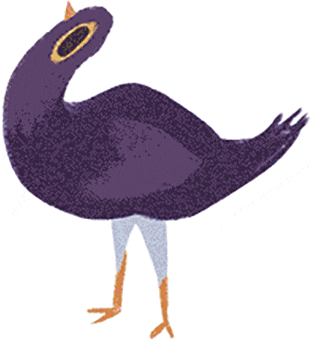
\includegraphics[width=3cm]{dove}
\caption{A pigeon.}
\end{figure}


\begin{proof}
Let $f$ be a monomorphism; suppose that $f$ is not surjective. Then there is a vector $w \in W$ such that $\forall v\in V,~w\ne f(v).$ Since $f(0)=0$, other vectors in $V$ are not mapped to 0 and hence $\ker f = \{0\}.$ And we get $\operatorname{dim}\operatorname{im}f = n$ from $\operatorname{dim}\ker  f = 0$. Hence $\operatorname{im}f = W.$

Changing im and ker proves the rest part of the theorem.
\end{proof}

Now we can prove the question in \textbf{Section 1.2}.

\begin{theorem}\label[thm]{t:matinv}
For two square matrices $A$ and $B\in\mathfrak M_{n,n}(F)$, if $AB=I$, then $A=B^{-1}.$
\end{theorem}
\begin{proof}
$AB=I$ implies that $B$ is left-invertible, which is equivalent to that $L_B$ is a monomorphism. Since $L_B:~F^n\to F^n$, $L_B$ is an isomorphism whence $B$ is invertible: $$B^{-1} = \begin{pmatrix} | & & | \\ L_B^{-1}\mathbf e_1 &\cdots & L_B^{-1}\mathbf e_n \\ | & & | \end{pmatrix}. $$ Multiplying $B^{-1}$ right in the both sides of $AB=I$, we obtain $A=B^{-1}.$ Similarly, $A$ is invertible and $A^{-1} = B.$
\end{proof}

\subsection{Rank}
\begin{defn}
For a matrix $A\in\mathfrak M_{m,n}(F),$ the \textbf{row space} is a space which is generated by the row vectors of $A.$ Similarly, the \textbf{column space} is a space which is generated by the column vectors of $A.$ Then the \textbf{row}(\textit{column}) \textbf{rank} is the dimension of the row(\textit{column}) space.
\end{defn}
\begin{ex}
We can know the row rank and the column rank in the (R, C)-REF of the matrix; one can do elementary row operations: \begin{align*}
A &= \begin{pmatrix}1&0&1\\5&6&7\\0&3&1\end{pmatrix}\\
&\sim_r \begin{pmatrix}1&0&1\\0&6&2\\0&3&1\end{pmatrix}\\
&\sim_r \begin{pmatrix}1&0&1\\0&6&2\\0&0&0\end{pmatrix}\\
&\sim_r \begin{pmatrix}1&0&1\\0&1&\frac 1 3 \\0&0&0\end{pmatrix};
\end{align*}
hence the row space is $\{(a,b,a+b/3)^\mathsf T:~a,b\in R\}$ whence the row rank is 2; while the column space is $\{(a+c,b+c/3,0)^\mathsf T = (\tilde a,\tilde b,0)^\mathsf T:~\tilde a,\tilde b\in R\}$ whence the column rank is also 2. Otherwise one can do elementary column operations: \begin{align*}
A &= \begin{pmatrix}1&0&1\\5&6&7\\0&3&1\end{pmatrix}\\
&\sim_c \begin{pmatrix}1&0&0\\5&6&2\\0&3&1\end{pmatrix}\\
&\sim_c \begin{pmatrix}1&0&0\\5&6&0\\0&3&0\end{pmatrix}\\
&\sim_c \begin{pmatrix}1&0&0\\0&1&0\\-\frac 5 2&\frac1 2&0\end{pmatrix};
\end{align*}
which makes the same result.
\end{ex}

Are the row rank and the column rank the same? The answer is...

\begin{lemma}For a matrix $A\in\mathfrak M_{m,n}(F)$ over an \emph{ordered field} $F$, $$\operatorname{col~rk}A = \operatorname{col~rk}A^\mathsf T.$$
\end{lemma}
\begin{proof}
It is suffices to show that $\operatorname{col~rk}A \le \operatorname{col~rk}A^\mathsf T,$ since it implies $$\operatorname{col~rk}A^\mathsf T \le \operatorname{col~rk}(A^\mathsf T )^\mathsf T  = \operatorname{col~rk}A$$which completes the proof of lemma.

We will show that $Av = 0$ if and only if $(A^\mathsf T A)v = 0$ whence $$\operatorname{col~rk}A = \operatorname{col~rk}(A^\mathsf T A) \le \operatorname{col~rk}A^\mathsf T$$; the last inequality follows because each column of $A^\mathsf T A$ is a linear combination of the columns of $A^\mathsf T$. First, $Av=0 \implies A^\mathsf T Av = 0$ trivially. Conversely, $$A^\mathsf T Av = 0 \implies v^\mathsf T A^\mathsf T A v = 0 \implies (Av)^\mathsf T Av = 0 \implies Av = 0,$$ by positive-definiteness of the dot product. (More generalized version of proof uses the orthogonal complement, or even \textbf{Erdős-Kaplansky Theorem}(?). See http://math.stackexchange.com/questions/2315/is-the-rank-of-a-matrix-the-same-of-its-transpose-if-yes-how-can-i-prove-it)\end{proof}
\begin{theorem}[rank theorem] The row rank and the column rank are the same, and we call it the \textbf{rank} of the given matrix.
\end{theorem}
\begin{proof}[Proof 1]
Count the number of \textit{leading 1} in RREF.
\end{proof}
\begin{proof}[Proof 2 assuming that $F$ is an ordered field]
It is trivial that the row rank of $A$ equals the column rank of $A^\mathsf T.$ Since the column rank of $A^\mathsf T$ is the same with of $A$, the proof completed.
\end{proof}
\begin{theorem}[rank-nullity theorem]
Let $A\in\mathfrak M_{m,n}(F)$ be a matrix, then $$\operatorname{rank}A + \operatorname{dim}\ker L_A = m.$$ We call $\operatorname{dim}\ker L_A$ the \textbf{nullity} of $A$, and denote $\operatorname{null}A$. Hence $$\operatorname{rank}A + \operatorname{null}A = m = \operatorname{dim}\operatorname{dom}L_A.$$
\end{theorem}
\begin{proof}
We know that $A\mathbf e_i$ is $i$-th column of $A$. Hence the column space of $A$ is just the image of $L_A:~F^m \to F^n$, hence $\operatorname{col~rk} A = \operatorname{dim}\operatorname{im}L_A.$ By the dimension theorem(\cref{t:dimthm}), $$\operatorname{dim}\ker L_A  + \operatorname{col~rk} A = \operatorname{dim} F^m = m.$$\end{proof}

\begin{defn}
Given an $m$ by $n$ matrix $A$ of rank $r$, a \textbf{rank decomposition} of $A$ is a representation by a product $A=PQ$ of two matrices $P\in\mathfrak M_{m,r}(F)$ and $Q\in\mathfrak M_{r,n}(F).$
\end{defn}
\begin{theorem}
A rank decomposition of a matrix exists, but not uniquely.
\end{theorem}
\begin{proof}
%%%%%%%%%%%%%%%%%%%%%%%%%%%%%%%%%%%%%%%%%%%%%%%%%%%%%%%%%%%%%%%%%%%%%%%%%%%5
\end{proof}


\subsection{Matrix representation and similarity}
\begin{defn}
For a finite dimensional vector space $V$ and a basis $\mathfrak B = \{v_i\}_{i\in I}$ of $V$, every vector $v$ in V can be represented as a linear combination of $\mathfrak B$ \textit{uniquely}, namely $$v = \sum a_i v_i;$$ and we call the row vector $$[v]_{\mathfrak B} = \begin{pmatrix}a_1 \\ \vdots \\ a_n\end{pmatrix}$$ the \textbf{coordinate} vector.
\end{defn}

\begin{theorem}
For a $F$-vector space homomorphism $f:~V\to W$ and the bases $\mathfrak B$ and $\mathfrak C$ of V and W, respectively, there is a unique matrix $[f]^{\mathfrak B}_{\mathfrak C} \in \mathfrak M_{\operatorname{dim}V,~\operatorname{dim}W}(F)$ such that $$[f]^{\mathfrak B}_{\mathfrak C} [v]_{\mathfrak B} = [fv]_{\mathfrak C}.$$
\end{theorem}
\begin{proof}
Let $n=\operatorname{dim}V$, $m=\operatorname{dim}W$, $\mathfrak B = \{ v_i\}_{i=1}^{n}$ and $\mathfrak C = \{ w_j\}_{j=1}^{m}$, then
\begin{align*}
\left[f(v)\right]_\mathfrak C &= \left[f\left(\sum_i a_i v_i \right) \right]_\mathfrak C
  \\ &= \left[\sum_i a_i f\left( v_i \right)\right]_\mathfrak C
  \\ &= \left[\sum_i a_i \sum_j b_{ij} w_j\right]_\mathfrak C
  \\ &= \left[\sum_j \left(\sum_i a_i b_{ij}\right) w_j\right]_\mathfrak C
  \\ &= \begin{pmatrix}\sum_i a_i b_{i1} \\ \vdots \\ \sum_i a_i b_{im}\end{pmatrix}
  \\ &= \begin{pmatrix}b_{11} & \cdots & b_{n1} \\ \vdots & \ddots & \vdots \\ b_{1m} & \cdots & b_{nm} \\ \end{pmatrix}\begin{pmatrix}a_1 \\ \vdots \\ a_n\end{pmatrix}
  \\ &= [f]^{\mathfrak B}_{\mathfrak C} [v]_\mathfrak B,
\end{align*} where $[f(v_i)]_\mathfrak C = [b_{i1} ~ \cdots ~ b_{im}]^\mathsf T$ whence $$[f]^\mathfrak B _ \mathfrak C = \bigg( [f(v_1)]_\mathfrak C ~~~ \cdots ~~~ [f(v_n)]_\mathfrak C \bigg).$$ Uniqueness follows from the uniqueness of the coordinate representation.
\end{proof}
\begin{prop}[composition and product] \label[prop]{p:comprod} Let $V \xrightarrow{f} W \xrightarrow{g} U$ be two homomorphisms. Then
$$[g\circ f]^\mathfrak B _ \mathfrak D = [g]^\mathfrak C _ \mathfrak D [f]^\mathfrak B _ \mathfrak C.$$
\end{prop}
\begin{proof}
Easy.
\end{proof}
Therefore, if the bases are fixed, there is a \textit{one-to-one correspondence} between the space of matrices and the space of linear transformations; where the operations are preserved under the correspondence, as follows: $$f+g \quad \longleftrightarrow \quad [f] + [g]$$ and $$f\circ g \quad \longleftrightarrow \quad [f][g].$$ We just say that, \begin{center}``the matrices are the same thing as the linear transformations.''\end{center}

\subsection{Basis transition}
\begin{theorem} Let $\mathfrak B$ be a basis of $F^n$ and let $A$ is an $n$ by $n$ square matrix. Then $A\mathfrak B = \{Av_i:~v_i\in\mathfrak B\}$ is a basis of $F^n$ if and only if $A$ is invertible.
\end{theorem}
\begin{proof}
Denote $\mathfrak B= \{v_i:~1\le i \le n\}$ like a column vector, although $F^n$ is not a field, namely, $$\mathfrak B = \begin{pmatrix} v_1\\ v_2 \\ \vdots \\ v_n \end{pmatrix}.$$ And define $A\mathfrak B$ as componentwise product: $$A\mathfrak B = \begin{pmatrix} Av_1\\ Av_2 \\ \vdots \\A v_n \end{pmatrix}.$$

($\Rightarrow$) If $Y$ is a basis, then $\exists C \in \mathfrak M_{n,n}(F),\quad C(A\mathfrak B) = \mathfrak B$ since $A\mathfrak B$ spans $F^n.$ $(CA)\mathfrak B = \mathfrak B$ implies that $(CA)v_i = v_i$ for every basis element $v_i \in \mathfrak B$ whence $CA = I$ and it implies that $A$ is invertible.

($\Leftarrow$) Let $v=\sum_i a_i v_i$ and $$R = \begin{pmatrix}a_1&\cdots&a_n\end{pmatrix}$$ be the coefficient matrix. Then $$v = \sum a_i v_i = R\mathfrak B = (R A^{-1})(A\mathfrak B) = \tilde R (A\mathfrak B)$$ whence $A\mathfrak B$ is a basis of $F^n$.
\end{proof}
\begin{theorem} \label[thm]{t:trninv}
If $\mathfrak B$ and $\tilde{\mathfrak B}$ are bases of V and $\mathfrak C$ and $\tilde{\mathfrak C}$ are bases of W, then for linear $f:~V\to W,$ $$[\operatorname{id}_W]_{\tilde{\mathfrak C }} ^{ \mathfrak C} [f]^{\mathfrak B}_{\mathfrak C} [\operatorname{id}_V]^{\tilde{\mathfrak B}} _{ \mathfrak B} = [f]^{\tilde{\mathfrak B}}_{\tilde{\mathfrak C}}.$$ Furthermore, $[\operatorname{id}]_\bullet^\bullet$ are all invertible.
\end{theorem}
\begin{proof}
For the first assertion, just use \cref{p:comprod}. For the second one, since $$[\operatorname{id}]_{\mathfrak B}^{\tilde{\mathfrak B}}[\operatorname{id}]^{\mathfrak B}_{\tilde{\mathfrak B}} = [\operatorname{id}]_{\mathfrak B}^{\mathfrak B} = I_{\operatorname{dim}\bullet},$$they are invertible by \cref{t:matinv}.

\end{proof}
\begin{prop}
For two bases $\mathfrak B$ and $\tilde{\mathfrak B}$ of $V$, the \textbf{transition matrix} $[\operatorname{id}_V]^\mathfrak B _{\tilde{ \mathfrak B}}$ is invertible. Conversely, for a basis $\mathfrak B$ of $V$ and an invertible square matrix $U$ whose the number of row is the dimension of the space $V$, there is a basis $\tilde{\mathfrak B}$ of $V$ such that $$U = [\operatorname{id}_V]^\mathfrak B _{\tilde{ \mathfrak B}}.$$
\end{prop}
\begin{proof}
The first assertion was proved in \cref{t:trninv}. For the second, let $$U = \begin{pmatrix}a_{11}&\cdots &a_{1n} \\ \vdots &\ddots &\vdots \\a_{n1}&\cdots&a_{nn} \end{pmatrix}$$ and $\mathfrak B = \{v_i\}$. We want another basis $\tilde{\mathfrak B} = \{w_i\}$ which satisfies $$U = [\operatorname{id}_V]^\mathfrak B _{\tilde{ \mathfrak B}} = \begin{pmatrix} | & & | \\ [v_1]_{\tilde{ \mathfrak B}} & \cdots & [v_n]_{\tilde{ \mathfrak B}} \\ | && | \end{pmatrix},$$ that is, $$v_i = \sum_{j} a_{ij}w_j, \qquad \begin{pmatrix} v_1 \\ \vdots \\ v_n \end{pmatrix} = \begin{pmatrix}a_{11}&\cdots &a_{1n} \\ \vdots &\ddots &\vdots \\a_{n1}&\cdots&a_{nn} \end{pmatrix}\begin{pmatrix} w_1 \\ \vdots \\ w_n \end{pmatrix} = U \begin{pmatrix} w_1 \\ \vdots \\ w_n \end{pmatrix} \qquad $$ Hence we have $$\tilde{\mathfrak B} = U^{-1}\mathfrak B.$$
\end{proof}
\subsection{Similarity}
\begin{defn}[similarity]
For two square matrices $A$ and $\tilde A$, we say those are \textbf{similar} if there is an invertible matrix $U$ such that $$\tilde A = U^{-1}AU,$$and denote $A\sim \tilde A$.
\end{defn}
\begin{prop}
Similarity relation is an \textbf{equivalence relation}, that is, satisfies the following three properties: \begin{itemize}
\item (Reflexivity) $A \sim A,$
\item (Symmetricity) $A \sim B \Longrightarrow B \sim A,$
\item (Transitivity) $A\sim B \sim C \implies A\sim C.$
\end{itemize}
\end{prop}

\begin{ex}[similarity]
For two square matrices $A$ and $\tilde A$, we say those are \textbf{similar} if there is an invertible matrix $U$ such that $$\tilde A = U^{-1}AU,$$and denote $A\sim \tilde A$.
\end{ex}
\begin{prop}
[similarity]
For a linear operator $f:~V\to V$ and the bases $\mathfrak B$, $\tilde{\mathfrak B}$ of $V$, two matrix representations of $f$ are similar, that is, $$[f]^{\mathfrak B} _{\mathfrak B} \sim [f]^{\tilde{\mathfrak B}} _{\tilde{\mathfrak B}}.$$
\end{prop}
\begin{proof}
$$[\operatorname{id}_V] _{\tilde{\mathfrak B}} ^{\mathfrak B} [f]^{\mathfrak B} _{\mathfrak B} [\operatorname{id}_V] ^{\tilde{\mathfrak B}} _{\mathfrak B} = [f]^{\tilde{\mathfrak B}} _{\tilde{\mathfrak B}}.$$
\end{proof}

\chapter{Matrix Group}
\section{Linear Groups}

\begin{defn}[normal subgroup]
A \textbf{normal subgroup} $N$ of a given group $G$ is a subgroup which left and right cosets $gN$ and $Ng$ are the same: $gN = Ng$, i.e., $$gNg^{-1} = N$$ for every $g\in G.$ We denote it as $N \triangleleft G$.
\end{defn}
\begin{prop}[why normal?] The quotient group $G/N$ (read $G$ mod $N$) is well-defined if and only if $N$ is normal of G.
\end{prop}
\begin{proof}
Whatever we take, the equivalence class must be the same. If $N$ is normal and letting $x\sim \tilde x$, i.e., $x^{-1}\tilde x \in N$, $$\tilde xN \subseteq (xN)N = xN$$ and \textit{vice versa}. If $\bar x = \bar{\tilde x} $ if $x\sim \tilde x$ and $\overline{xy} = \bar x \bar y,$ we have $$gN = (1g)N = NgN = hNgN = (hg)N$$ for every $h\in N$, hence $N = g^{-1} hgN$ so that $N$ is normal: letting $n = g^{-1}hg\tilde{n}$, we have $g^{-1}hg=n\tilde{n}^{-1}\in N$ for every $h\in N$ whence $g^{-1}Ng \subseteq N.$
\end{proof}
\begin{defn}[general linear group and special linear group] The \textbf{general linear group} of a given vector space $V$ is a (multiplicative) group of automorphism on $V$; that is, $\operatorname{GL}(V) = \mathfrak L(V,V)^\times.$ And the \textbf{special linear group} of $V$ is the subgroup of $\operatorname{GL}(V)$ which is consisted by linear transformations whose determinant are all 1.

We denote $\operatorname{GL}(n, F) = \operatorname{GL}(F^n),$ and $\operatorname{SL}(n, F) = \operatorname{SL}(F^n).$
\end{defn}
\begin{theorem}[first isomorphism theorem]
For any homomorphism $\varphi:~G\to H$ for two groups $G$ and $H$, $$G/\ker \varphi \approx \operatorname{im} \varphi.$$
\end{theorem}
\begin{proof}
\hfill
\begin{center}
\leavevmode
\xy
\xymatrix {
G \ar@{->}[rr]^{\varphi} \ar@{->}[dr] &&\operatorname{im}\varphi\\ & G/\operatorname{ker}\varphi \ar@{->}[ur]_{\approx} &\\
}
\endxy
\end{center}
\end{proof}
\begin{prop}[GL and SL] $$\operatorname{GL}(V)/\operatorname{SL}(V) \approx F^\times.$$
\end{prop}

\begin{defn}[center] The \textbf{center} $Z(G)$ of a group $G$ is the subgroup of elements which satisfy the `commutative law', i.e., $$Z(G) = \{z\in G: \quad zg = gz \textrm{ for every }g\in G\}.$$ $Z$ for \textit{zentrum}, which means `center' in German.
\end{defn}
\begin{prop}[normality of the center]
$$Z(G)\triangleleft G.$$
\end{prop}
\begin{proof}
Trivially, $$gZ(G) = \{gz:~z\in Z(G)\} = \{zg:~z \in Z(G)\} = Z(G)g.$$
\end{proof}
\begin{ex}
What are the centers of (a) $\operatorname{GL}(n, F)$ and (b) $\operatorname{SL}(n, F)$?

Answer: (a) $0\ne cI$'s, (b) $\alpha I$'s where $\alpha^n = 1.$
\end{ex}
\begin{proof}
(a) is just all. Let $AZ = ZA$ for all invertible $A.$ Then, especially, for all \textit{elementary matrices}, $EZ = ZE.$ Note that multiplying $E$ left is the same with elementary \textit{row} operating, while multiplying right is for elementary \textit{column} operating. (Especially, for $E_{i + cj}$'s.) Hence we obtain that $Z$ is diagonal. Instead a more detailed explanation, we see an example: $$
\begin{pmatrix}
1 & 3 \\
0 & 1
\end{pmatrix}
\begin{pmatrix}
a & *_1 \\
*_2 & b
\end{pmatrix}
=
\begin{pmatrix}
a + 3*_2 & *_1 + 3b \\
*_2 & b
\end{pmatrix},$$
$$\begin{pmatrix}
a & *_1 \\
*_2 & b
\end{pmatrix}
\begin{pmatrix}
1 & 3 \\
0 & 1
\end{pmatrix}
=
\begin{pmatrix}
a  & *_1 + 3a \\
*_2 & b + 3*_2
\end{pmatrix},$$
hence $*_1$ and $*_2$ are zero. Similar details says that $Z$ must be diagonal, for bigger matrices.

Now, the proof is done: since $E_{i\leftrightarrow j}$ is an elementary matrix, $Z_{ii} = Z_{jj}$, for every $i$ and $j$ pair. Therefore $Z$ is a `nonzero'(since $Z$ is invertible!) multiple of $I.$

Not so surprisingly, the proof works on any \textit{ring} with 1; if we modify `nonzero' to `invertible', that is, $c\in R^{\times}.$
\end{proof}
\begin{add}[divide by center?] Dividing by center means to ignore the difference due to the elements of $Z.$ Since $$Z(G) = \{z\in G:\quad z = gzg^{-1}\textrm{ for every }g\in G\},$$ we have some `morphisms' $\varphi_g:~a \mapsto b = gzg^{-1}$ and \textit{their group} $$\operatorname{Inn}(G) = \{ \varphi_g:\quad g \in G\}.$$ We call this group the \textbf{inner automorphism group} of $G$.

We want to show that $G/Z(G) \approx \operatorname{Inn}(G).$ The idea is easy: use the homomorphism $\varphi_\bullet$ above: $$\varphi_\bullet:\quad G \to \operatorname{Inn}(G).$$ The kernel of this homomorphism is just the center of $G$, since the (multiplicational) identity of $\operatorname{Inn}(G)$ is the identity function $\operatorname{id}_G$ and, from $$\varphi_z = z\bullet z^{-1} = \operatorname{id}_G, \qquad \forall g\in G,$$i.e., $$\varphi_z (g) = zgz^{-1} = g, \qquad \forall g\in G,$$ we get $zg = gz$ whence $z \in Z(G).$ Therefore $\ker (\varphi_\bullet) = Z(G)$, and by the first isomorphism theorem, we obtain $$G/Z(G) \approx \operatorname{Inn}(G).$$
\end{add}

\begin{defn}[PGL and PSL]
The \textbf{projective general linear group} is defined by $$\operatorname{PGL}(V) = \operatorname{GL}(V)/Z(\operatorname{GL}(V)).$$
The \textbf{projective special linear group} is defined by $$\operatorname{PSL}(V) = \operatorname{SL}(V)/Z(\operatorname{SL}(V)).$$
\end{defn}

Projective geometry is difficult...

\section{Orthogonal group}
\begin{defn}[orthogonal transformation]
For an \textit{inner product space} $(V,~\langle \bullet , \bullet \rangle)$ (or even just a quadratic space with non-degenerate symmetric bilinear form), an \textbf{orthogonal transformation} of $V$ is an invertible linear transformation which preserves the given inner product, that is, such $A\in \operatorname{GL}(V)$: $$\langle v, ~w \rangle = \langle Av,~ Aw \rangle.$$ The group of such transformations is called the \textbf{orthogonal group} $\operatorname{O}(V)$ of $V$, and also denote $\operatorname{O}(n, F) = \operatorname{O}(F^n)$ and $\mathrm O(n) = \mathrm O(n, \mathbb R)$. $F^n$ is considered with \textit{dot product.}

Similarly, $\operatorname{SO}(V) = \{T\in \operatorname{O}(V):~ \operatorname{det}T = 1\}$, and analogous definitions for $\operatorname{SO}(n,F)$ and $\operatorname{SO}(n).$ Obviously, it is called the \textbf{special orthogonal group} of $V$.
\end{defn}
\begin{defn}[unitary group]
If we give a \textit{hermitian form} $(V, ~ \langle \bullet, \bullet \rangle )$ rather than an inner product, where the given field is `trivially' the field $\mathbb C$ of complex number, we define analogously \textbf{unitary group} $\operatorname{U}(n)$ as we defined the orthogonal group:$$\langle v, ~w \rangle = \langle Av,~ Aw \rangle, \qquad A \in \operatorname{GL}(n,~\mathbb C).$$ We \textit{already know} what is $\operatorname{SU}(n)$ and how to call it \textsf{:D}.
\end{defn}

\begin{prop}
\hfill
\begin{itemize}
    \item $\operatorname{SO}(V) \triangleleft\operatorname{O}(V) \triangleleft \operatorname{GL}(V);$
    \item $\operatorname{SO}(V) \triangleleft\operatorname{SL}(V) \triangleleft \operatorname{GL}(V);$
    \item $\operatorname{O}(n, F) = \{ A\in \mathfrak M_{n,n}(F)^\times:~ A^{-1}=A^\mathsf T\},$ if the inner product is a standard one, so-called \textit{dot product}. (\textit{Canonically isomorphic!})
\end{itemize}
Also the followings hold: for $\operatorname{O}(n, F)$,  every element is a matrix with pairwise orthonormal columns (or rows).
\end{prop}
Good, well, why it is called `orthogonal'? It is because these preserves the `angle' of two vectors, especially the \textit{orthogonality}. Then, \textit{what} is orthogonal? Which matrices are orthogonal?
\begin{prop}
\hfill

In $\mathbb R^2$, $\operatorname{O}(2)$ consists of rotations and reflections. And the group of rotations is just $\operatorname{SO}(2).$
\begin{proof}From
$$A=\begin{pmatrix}a&b\\c&d\end{pmatrix}, \qquad AA^\mathsf T = \begin{pmatrix}a&b\\c&d\end{pmatrix}\begin{pmatrix}a&c\\b&d\end{pmatrix} = \begin{pmatrix}a^2+b^2&ac+bd\\ac+bd&c^2+d^2\end{pmatrix} = I,$$
we obtain $a^2 + b^2 = 1 = c^2 + d^2$ and $ac+bd = 0$. Solutions for the first equality are just sines and cosines, namely: $$a = \cos x, ~~b = \sin x, \quad c = \cos y,~~d = \sin y.$$ (Orders of sine and cosine do not have to consider; since there is an inversion $\theta~\mapsto~\frac \pi 2 - \theta$.) Evaluating to another equality, $$\cos x \cos y + \sin x \sin y = \cos(y-x) = 0,\qquad y-x = \frac{2k-1}{2}\pi.$$ Hence $y = x + \frac{2k-1}{2}\pi.$ Substituting it, we get $$c = - \sin x \sin \left(\frac{2k-1}{2}\pi\right) = \mp \sin x,\qquad d = \cos x \sin \left(\frac{2k-1}{2}\pi\right) = \pm \cos x.$$ Due to a \textit{custom} in math and other sciences, we use $\theta = -x$ and finally get $$A=\begin{pmatrix}\cos \theta &-\sin \theta \\ \pm \sin \theta & \pm \cos \theta \end{pmatrix}.$$

If the signa of second row are pluses, $$A_+ = \begin{pmatrix}\cos \theta &-\sin \theta \\\sin \theta & \cos \theta \end{pmatrix} = R_\theta,$$ where $R_\theta$ is the \textbf{rotation matrix} of angle $\theta$. Since $ \operatorname{det}R_\theta = 1$, $R_\theta \in \operatorname{SO}(2).$

If the signa of second row are minuses, $$A_- = \begin{pmatrix}\cos \theta &-\sin \theta \\-\sin \theta & -\cos \theta \end{pmatrix}  = \begin{pmatrix}1&0\\0&-1\end{pmatrix} \begin{pmatrix}\cos \theta &-\sin \theta \\\sin \theta & \cos \theta \end{pmatrix} =\begin{pmatrix}1&0\\0&-1\end{pmatrix} R_\theta = S_{-\theta/2},$$ where $S_\varphi$ is a \textbf{reflection matrix} w.r.t. a line $\theta = \varphi$ in polar coordinate system. (Draw it $\sim \!.$) Note that $\operatorname{det}S_\varphi = -1$.
\end{proof}
\end{prop}

How about 3-dimensional space? We consider a rotation on a line, the \textit{axis}. For example, there are `basic' three rotations: $$\displaystyle {\begin{alignedat}{1}R_{x}(\theta )&={\begin{pmatrix}1&0&0\\0&\cos \theta &-\sin \theta \\[3pt]0&\sin \theta &\cos \theta \\[3pt]\end{pmatrix},}\\[6pt]R_{y}(\theta )&={\begin{pmatrix}\cos \theta &0&\sin \theta \\[3pt]0&1&0\\[3pt]-\sin \theta &0&\cos \theta \\\end{pmatrix},}\\[6pt]R_{z}(\theta )&={\begin{pmatrix}\cos \theta &-\sin \theta &0\\[3pt]\sin \theta &\cos \theta &0\\[3pt]0&0&1\\\end{pmatrix}.}\end{alignedat}}$$ Surprisingly, they are almost \textit{all}, i.e., the following holds. (Details are omitted.)

\begin{theorem}[decomposition of rotation]
For every `rotation' $R\in\operatorname{SO}(3)$,
$$R=R_{z}(\alpha )\,R_{y}(\beta )\,R_{x}(\gamma )\,$$
 where \textit{Tait-Bryan angles} of $R$ are $\alpha$, $\beta$, $\gamma$, about axes $z$, $y$, $x$ respectively.
\end{theorem}

Following our knowledge, there efinition for \textit{arbitrary rotation} is quite obvious, and only acceptable:

\begin{defn}[rotation] \textbf{Rotation} is an element of SO.\end{defn}

We must figure out the following definitions.
\begin{defn}[PGO, PSO, PGU, PSU]Projective (general) orthogonal group $\operatorname{PGO}(V)$ and projective special orthogonal group $\operatorname{PSO}(V).$ Similarly for U's...
\end{defn}
\begin{ex}
Calculate them! What is $Z(\operatorname{O}(V))$ and $Z(\operatorname{SO}(V))$?
\end{ex}
\begin{proof}
Same with \textbf{Example 1.1.} A difference is that $\det Z = \pm 1$ in $\operatorname{O}(V).$ Another one is for $\operatorname{SO}$: for odd-dimensional $V$, $Z(\operatorname{SO}(V))=\{I\}$ (a trivial group) since $\operatorname{det}\pm I = \pm 1$; while $Z(\operatorname{SO}(V))=\{\pm I\}$ for even-dimensional $V$ since $\operatorname{det}\pm I = 1.$
\end{proof}
\begin{coro}
\emph{PSO $\approx$ SO} for odd-dimensional vector space $V$.
\end{coro}
\begin{prop}
$$\operatorname{PSU}(2)\approx \operatorname{SO}(3), \qquad \operatorname{SU}(2) \dhxrightarrow{\text{double}} \operatorname{SO}(3),$$ where $\dhxrightarrow{\text{double}}$ means that there is a double covering.
\end{prop}

``The shortest path between two truths in the real domain passes through the complex domain.'' ---Jacques Hadamard.

\begin{proof}
$Z(\operatorname{SU}(2)) = \{\pm I\}$? Trivial. Then it suffices to show that $\operatorname{PSU}(2)\approx \operatorname{SO}(3)$. A transformation $A$ of $\operatorname{PSU}(2)$ satisfies \textsf{(U)} $AA^\dagger = I$ by the definition. Use same method as \textbf{Proposition 1.5.}: let $$A=\begin{pmatrix}a&b\\c&d\end{pmatrix},$$ then $$AA^\dagger = \begin{pmatrix}a&b\\c&d\end{pmatrix}\begin{pmatrix}\bar a&\bar c\\\bar b&\bar d\end{pmatrix} = \begin{pmatrix}a\bar a+b\bar b&a\bar c+b\bar d\\\bar a c+\bar b d&c\bar c + d\bar d\end{pmatrix}=I$$ whence $$|a|^2 + |b|^2 = 1 = |c|^2 + |d|^2, \qquad a\bar c + b\bar d = 0.$$ The first equality gives us $$a = e^{i\varphi_1}\cos x,~~b = e^{i\varphi_2}\sin x,~~c = e^{i\varphi_3}\cos y,~~d = e^{i\varphi_4}\sin y,$$ and the second equality gives $$\cos x \cos y + e^{i(-\varphi_1+\varphi_2+\varphi_3-\varphi_4)}\sin x \sin y = 0,$$ since $\overline{e^{i\theta}} = e^{-i\theta}$ for real $\theta$. If $-\varphi_1+\varphi_2+\varphi_3-\varphi_4 \ne 0,$ the equality must not hold unless $b=d=0$, which leads to a contradiction. Also, since \textsf{(S)} $\operatorname{det}A = 1$, $$ad-bc = e^{i(\varphi_1 + \varphi_4)}(\cos x \sin y - \sin x \cos y) = e^{i(\varphi_1 + \varphi_4)} \sin(y-x) = 1$$ whence $\varphi_1 + \varphi_4 =\varphi_2 + \varphi_3 = k\pi$ and $y-x = \frac{2k-1}{2} \pi.$ Therefore $$A = \begin{pmatrix}e^{i\varphi_1}\cos x&e^{i\varphi_2}\sin x \\ \mp e^{- i\varphi_2}\sin x&\pm e^{-i\varphi_1}\cos x \end{pmatrix}.$$ Finally, \textsf{(P)} ignore one signum of them, then we have $$A = \begin{pmatrix}e^{i\varphi_1}\cos \theta & - e^{i\varphi_2}\sin \theta \\  e^{- i\varphi_2}\sin \theta& e^{-i\varphi_1}\cos \theta \end{pmatrix}.$$ Hence, for example, there is an `isomorphism' $$\begin{pmatrix}e^{i\varphi_1}\cos \theta & - e^{i\varphi_2}\sin \theta \\  e^{- i\varphi_2}\sin \theta& e^{-i\varphi_1}\cos \theta \end{pmatrix} \leftrightarrow (\theta, \varphi_1, \varphi_2) \leftrightarrow R_z(\theta)R_y(\varphi_1)R_x(\varphi_2),$$ since $R_\bullet (\alpha + \beta) = R_\bullet (\alpha)R_\bullet (\beta).$ Therefore $\operatorname{PSU}(2)\approx \operatorname{SO}(3).$
\end{proof}
\section{SO(1,1)}
\begin{defn}[indefinite orthogonal group] Consider the Euclidean space only, i.e.,   $F=\mathbb R$.
The \textbf{indefinite orthogonal group} $\operatorname{O}(p, q)$ is something like O, but the inner product is not provided while the following bilinear form is given: $$\langle v, w\rangle = v^\mathsf T \operatorname{diag}(\underbrace{1, \cdots, 1}_{p}, \underbrace{-1, \cdots, -1}_{q}) w,$$
 for $(p+q)$-dimensional vectors $v$ and $w$. For instance, $\operatorname{O}(n) = \operatorname{O}(n,0) = \operatorname{O}(0,n).$
And SO$(p,q)$ is ...
\end{defn}
We are interested in O(1,1) and O(1,3) in particular.
\begin{prop}
$\operatorname{SO}(1,1)$ can be represented by a hyperbolae $x^2 - y^2 = 1$, hence 2 connected curves. $\operatorname{SO}^+$ is the `connected' component of this group which contains the identity $I$, $$\operatorname{SO}^+ = \left\{ \begin{pmatrix}\cosh \theta & \sinh \theta \\ \sinh \theta & \cosh \theta\end{pmatrix}:~~ \theta\in\mathbb R \right\}.$$ In fact, we call the connected component of a given `topological' group that contains the identity element the \textbf{identity component} of given group.
\end{prop}
\begin{center}

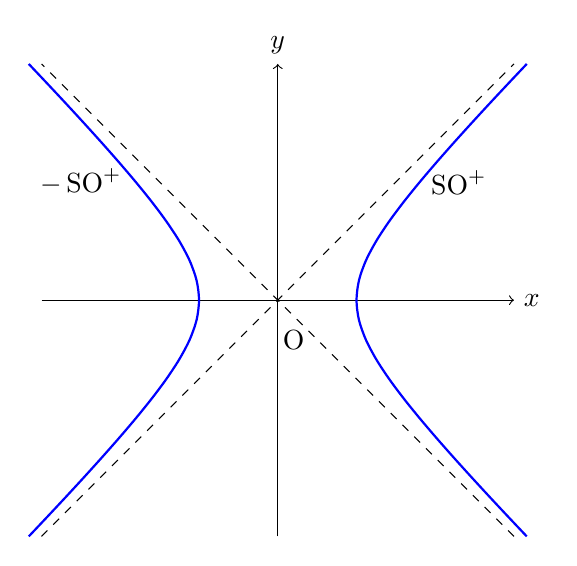
\begin{tikzpicture}
\draw[->] (-3,0) -- (3,0) node[right] {$x$};
\draw[->] (0,-3) -- (0,3) node[above] {$y$};
\draw[dashed] (-3,-3) -- (3,3);
\draw[dashed] (3,-3) -- (-3,3);
\draw[scale=1,domain=-3:3,smooth,variable=\y,blue,thick] plot ({(\y*\y + 1)^(1/2)},{\y});
\node at (2.3,1.5) {$\operatorname{SO}^{+}$};
\draw[scale=1,domain=-3:3,smooth,variable=\y,blue,thick] plot ({-(\y*\y + 1)^(1/2)},{\y});
\node at (-2.5,1.5) {$-\operatorname{SO}^{+}$};
\node at (0.2,-0.5) {O};
\end{tikzpicture}
\end{center}
\begin{proof}
Completely same process. Note that if $A\in\operatorname{SO}(1,1)$, $$v^\mathsf T \begin{pmatrix}1&0\\0&-1\end{pmatrix}w = \langle v,w\rangle = \langle Av,Aw\rangle =v^\mathsf T A^\mathsf T \begin{pmatrix}1&0\\0&-1\end{pmatrix}Aw,$$ hence $$\begin{pmatrix}1&0\\0&-1\end{pmatrix} = A^\mathsf T \begin{pmatrix}1&0\\0&-1\end{pmatrix} A.$$ Then we have $$\operatorname{SO}(1,1) = \left\{ \pm \begin{pmatrix}\cosh \theta & \sinh \theta \\ \sinh \theta & \cosh \theta\end{pmatrix}:~~ \theta\in\mathbb R \right\}.$$ We \textit{can(?)} represent it as a parametrized hyperbola: $$\pm \begin{pmatrix}\cosh \theta & \sinh \theta \\ \sinh \theta & \cosh \theta\end{pmatrix} \longleftrightarrow \pm\begin{pmatrix}\cosh \theta\\ \sinh \theta\end{pmatrix},$$ then $\operatorname{SO}^+$ and $-\operatorname{SO}^+$ are connected components of $\operatorname{SO}(1,1).$
\end{proof}
What does `connected' means? Detail definition is in \textit{topology}: it cannot separated by some open sets.

We will stop our work here about groups for the time being. If we learn \textit{topology} or \textit{Lie group theory}, it will continue...

\chapter{Similarity}
\section{Eigen-\textit{something}}
The prefix \textit{eigen}- is adopted from the German word \textit{eigen} for ``own-" or ``unique to", ``peculiar to". We will study about some \textit{unique} something, up to similarity.

\begin{defn}[eigenvalue, eigenvector, eigenspace] For a linear \textit{operator} $T \in \mathfrak L(V,V)$, if $$Tv = \lambda v$$ for a scalar $\lambda\in F$ and a \textit{nonzero} vector $v\in V$, we call $\lambda$ an \textbf{eigenvalue} and $v$ an \textbf{eigenvector} of $T$. The \textbf{eigenspace} of $\lambda$ is a subspace $$E_\lambda = \left \{v\in V: ~~ Tv= \lambda v\right\} = \ker(T-\lambda I)$$ of all vectors whose eigenvalue is $\lambda$.
\end{defn}
\begin{ex}
Check whether $E_\lambda$ is a subspace of $V$.
\end{ex}
\begin{prop}
If $f(t) \in F[t]$ and $v\in E_\lambda$, then $f(T)v = f(\lambda)v.$
\end{prop}
\begin{theorem}
TFAE(the followings are equivalent):
\begin{enumerate}[label={(\alph*)}]
    \item $\lambda$ is an eigenvalue of $T$.
    \item $T-\lambda I$ is singular, i.e., non-invertible.
    \item $\operatorname{det} (T-\lambda I) = 0.$
\end{enumerate}
\end{theorem}
\begin{proof}
We already(and MUST) know that (b) and (c) are equivalent. If $T-\lambda I$ is invertible, $$Tv = \lambda v ~~~~\Longleftrightarrow~~~~ (T-\lambda I)v = 0~~~~\Longleftrightarrow~~~~v=0$$and hence $\lambda$ is not an eigenvalue. And if $\lambda$ is an eigenvalue, $T-\lambda I$ is not bijective and hence singular.
\end{proof}
Thus, determinant of $\lambda I - T$ is important to decide whether or not $\lambda$ is an eigenvalue of $T$. Hence we define a \textit{polynomial}:
\begin{defn}[characteristic polynomial] The \textbf{characteristic polynomial} $\phi_T(t)$ is a polynomial defined by $$\phi_T(t) = \operatorname{det} (tI-T).$$ We will write $\chi\phi$ instead of the term `characteristic polynomial' since it is so long. \textsf{XD}

Here, $t$ behaves like a \textit{scalar} since it used instead of a scalar $\lambda$.
\end{defn}
Note that $\lambda$ is an eigenvalue iff $\phi_T (\lambda) = 0.$
\begin{ex}
Check if $\chi\phi$ is really a polynomial.
\end{ex}
\begin{ex}
Calculate the $\chi\phi$ of a matrix $$A = \begin{pmatrix}3&3&-1\\2&2&-1\\2&2&0\end{pmatrix}.$$ Find its eigenvalues and eigenspaces, and calculate $\phi_A (A)$. Note that $$f(T) = \sum a_n T^n$$ for a polynomial $f(t) = \sum a_n t^n \in F[t]$ and a linear operator $T$. \label[ex]{ec}
\end{ex}

\section{Diagonalizability}

Why we consider it? A big \textit{raison d'etre} of eigen-something is \textit{diagonalization} of a linear operator. First, from its name, we can define as follows:

\begin{defn}[diagonalization]
A \textbf{diagonalization} of a linear operator $T\in \mathfrak L(V,V)$ is a representation $T$ as a similar operator of a diagonal operator $D = \operatorname{diag}(d_1,\cdots,d_n).$ If there is a diagonalization of $T$, that is $T\sim D$ for a diagonal operator $D$, then we call $T$ is \textbf{diagonalizable}.
\end{defn}
\begin{ex}
Determine whether the following matrices are diagonalizable, where $F=\mathbb Q$:
$$A=\begin{pmatrix} -1 & 3 & -1 \\ -3 & 5 & -1 \\ -3 & 3 & 1 \end{pmatrix},\qquad B= \begin{pmatrix} 0 & 1 \\ -1 & 0 \end{pmatrix}. $$ If a matrix is not diagonalizable in given field, consider $F=\mathbb R$ and $F=\mathbb C$.
\end{ex}

If $T$ is diagonalizable, then $[T]_{\mathfrak B}^{\mathfrak B} = U^{-1}DU$ for a diagonal matrix $D$, supposing the basis $\mathfrak B$ is given for the vector space $V$; and there is another basis $\mathfrak C$ for $V$ such that $U = [\operatorname{id}_V]_{\mathfrak B}^{\mathfrak C}$. Evaluating this, we obtain $D=[T]_{\mathfrak C}^{\mathfrak C}.$ Since it is diagonal, we have $$[D]^{i} = D\mathbf e_i  = [T]_{\mathfrak C}^{\mathfrak C} [w_i]_{\mathfrak C}=[T w_i]_{\mathfrak C}$$ and $$D\mathbf e_i = d_i\mathbf e_i =[d_i w_i]_{\mathfrak C},$$ where $D=\operatorname{diag}(d_1,\cdots,d_n)$ and $\mathfrak C = \{w_1, \cdots, w_n\}.$ Hence we have $Tw_i = d_i w_i$, i.e., new basis must consist of eigenvectors, and the diagonal matrix contains corresponding eigenvalues. It is equivalent to the original definition. Hence we can re-define diagonalizability of a linear operator without matrices:
\begin{defn}[redefine of diagonalizability] A linear operator $T\in\mathfrak L(V,V)$ is diagonalizable if there is a basis for $V$ whose elements are all eigenvectors of $V$.
\end{defn}
Since eigenvectors span $V$, there are $n$ linearly independent eigenvectors.
\begin{prop}
If the eigenvalues of $T$ are mutually different, $T$ is diagonalizable.
\end{prop}
\begin{proof}
If $\lambda$'s are different, eigenvectors are linearly independent.
\end{proof}
\begin{prop}
If $H$ is Hermitian, that is $H=H^\dagger$, then $H$ can be diagonalized by a unitary operator $U$, i.e., $U^{-1} = U^\dagger.$
\end{prop}
\begin{proof}
Exercise.
\end{proof}
\begin{theorem}
Let $T\in \mathfrak L(V,V)$ and $\lambda_i$'s are eigenvalues of $T$. Then TFAE:
\begin{enumerate}[label={(\alph*)}]
    \item $T$ is diagonalizable,
    \item $\phi_T(t) = \prod (x-\lambda_i)^{e_i}$, $e_i = \dim E_{\lambda_i},$
    \item $V = \bigoplus E_{\lambda_i},$
    \item $\dim V = \sum \dim E_{\lambda_i}.$
\end{enumerate}
\end{theorem}
\begin{proof}
\begin{description}
\item [(a)$\Rightarrow$(b)] $\chi\phi$ is invariant under similarity, since $$tI - T = U^{-1}(tI - D)U,$$for example. Hence $$\phi_T(t) = \phi_D(t) = \prod (t-\lambda_i)^{e_i}.$$ A term due to a basis element appears once in the characteristic polynomial, hence the exponent of $t-\lambda_i$ is the (maximum) number of independent vectors in $E_{\lambda_i}$, i.e., dimension.
\item [(b)$\Rightarrow$(c)$\Rightarrow$(d)$\Rightarrow$(a)] ㅎㅎ. For (b) to (c), use dimension argument. Note that $\sum e_k = n$.
\end{description}
\end{proof}

\section{Cayley-Hamilton Theorem and Minimal Polynomial}

From \cref{ec}, we can know $\phi_A (A)$ for some matrices. Is it a general result? The answer is \textsf{YES}, and it is called \textit{Cayley-Hamilton theorem}!
\begin{theorem}[Cayley-Hamilton] $$\phi_T(T)=0.$$\end{theorem}
For $n=2$, let $A = \begin{pmatrix}a&b\\c&d\end{pmatrix}.$ Then $$\phi_A(t) = (t-a)(t-d)-bc = t^2 - (a+d)t + (ad-bc)$$ and we get a \textit{familiar}(?) form: $$T^2 - (a+d)T + (ad-bc)=0.$$
\begin{proof}[Proof(?)] Evaluating $t=T$, $$\phi_T(T) = \det(TI-T) = \det(T-T) = 0.$$

(\textbf{NOT A PROOF.}) \renewcommand{\qedsymbol}{$\lightning$}
\end{proof}
First, $t$ behaves as a scalar. And also $0$ is a zero matrix, rather than a scalar 0, in a formula $\phi_T(T)=0.$

Then how to prove it? We will consider $t^n \phi_T(t^{-1})$.

\begin{proof} Let $\phi_T(t) = \sum_{i=0}^n c_i t^i,$ then
  $$t^n \phi_T(t^{-1}) = \sum_{i=0}^n c_i t^{n-i}
  = t^n \operatorname{det}\left( t^{-1}I-T \right)
  = \operatorname{det}(I-tT).$$
From $$\operatorname{det}(A)I = A \cdot \operatorname{adj}A,$$
we get $$\operatorname{det}(I-tT)I = (I-tT)\operatorname{adj}(I-tT).$$
In order to `remove' $I-tT$ in the RHS, multiplying $\sum_{i=0}^m(tT)^i $ left,
$$\begin{aligned}\left(\sum_{i=0}^m (tT)^i \right) \left(\sum_{i=0}^n c_i t^{n-i}\right) &=
\left(\sum_{i=0}^m (tT)^i \right) \operatorname{det}(I-tT)I \\ &=
 \left(\sum_{i=0}^m (tT)^i \right) (I-tT)\operatorname{adj}(I-tT) \\ &
 = \left(I-(tT)^{m+1} \right) \operatorname{adj}(I-tT).\end{aligned}$$
By definition of classical adjoint, every entry of this matrix is a polynomial
of degree less than $n$. Hence RHS have terms of degree less than $n$ or greater
than or equal to $m$; for big $m$, the terms of degree $d\in [n,m)$ in LHS must
be vanished. Hence, with $m$ big enough, we obtain that the coefficient of the term of degree $n$ is zero. Now, observing the coefficient
of the term of degree $n$, we get
$$\sum_{i=0}^n c_i T^i = 0.$$
Hence $\phi_T(T) = 0.$
\end{proof}

\begin{defn}[annihilating ideal]
$$\mathcal I_T = \{p(t) \in F[t]:~~p(T) = 0\}.$$
A polynomial in $\mathcal I_T$ is called an \textbf{annihilating polynomial}.
\end{defn}
Since $\phi_T(t) \in \mathcal I_T$, by Cayley-Hamilton theorem, $\mathcal I_T \ne \emptyset.$
\begin{theorem}[minimal polynomial]
There is a monic annihilating polynomial which has the smallest degree. `Monic' means that the coefficient of the highest order term is 1. We call this polynomial the \textbf{minimal polynomial} $m_T(t).$ And also, $$m_T(t) | p(t), \qquad p(t) \in \mathcal I_T;$$especially, $m_T(t) | \phi_T(t).$
\end{theorem}
\begin{proof}
  Since $\operatorname{deg}\mathcal I_T$ is a subset of $\mathbb N$, there is the minimal degree $d$. If there is two different monic annihilating polynomial of degree $d$, denoting $m_1$ and $m_2$, we have $m_1 - m_2 \in \mathcal I_T$ which leads to a contradiction.
  
  If $m_T(t) \not\!|\; p(t)$ for every $p(t)\in\mathcal I_T,$ by division algorithm, we get that the remainder $r(t) = p(t)~\textrm{mod}~m_T(t)$ is also an annihilating polynomial which has the degree less than of $m_T(t),$ a contradiction.
\end{proof}
\begin{prop}
$\mathcal I_T$ is really an ideal. (Of a ring $F[t].$)
\end{prop}
\begin{proof}
  Exercise.
\end{proof}
\begin{ex}
Find the $\chi \phi$ and $m\phi$ of a matrix $$A=\begin{pmatrix}5&-6&-6\\-1&4&2\\3&-6&-4\end{pmatrix}.$$
\end{ex}
\begin{proof}[Answer]
$$\phi_A(t) = (t-1)(t-2)^2 ,\qquad m_A(t) = (t-1)(t-2).$$
\end{proof}
\section{Invariant and Triangularizability}
\begin{defn}[invariant subspace]
  For $T\in\mathfrak L(V,V)$ and $W\le V$, $W$ is called invariant under $T$ if $TW \le W.$
\end{defn}
\begin{ex}
  \begin{itemize}
    \item $F[t]$ is invariant under $D = \frac{\mathrm d}{\mathrm dt}.$
    \item Every space is invariant under a projection.
    \item Suppose there are two linear operator $T$ and $S$ on $V$, which commute, i.e., $TS = ST$. Let $W = \operatorname{im} S$ and $N = \ker S$, then $W$ and $N$ are invariant under $T$, since $TW = TSV = STV \le SV = W$ and $Sn = 0 \implies STn = TSn = 0.$
  \end{itemize}
\end{ex}
Let $W\le V$ be invariant under $T$, and $\mathfrak C = \{w_i\}_{i=1}^m$ be a basis of $W$. Then, $$[T]_{\mathfrak C}^{\mathfrak C} = \begin{pmatrix}[T\upharpoonright _W]^{\mathfrak C}_{\mathfrak C} & * \\ \mathbf 0 & *\end{pmatrix},$$ since, letting $\mathfrak B = \{w_i, v_j\}_{i=1,j=1}^{m,~n-m}\supseteq \mathfrak C$ be a basis of $V$, $$Tw_i = \sum a_iw_i + \sum 0 v_j.$$

\begin{theorem}
  Let $W\le V$ be invariant under $T$, then $$\phi_{T\upharpoonright _W} | \phi_T\qquad \textrm{and}\qquad m_{T\upharpoonright W} | m_T.$$
\end{theorem}
\begin{proof}
Let $W$ has a basis $\mathfrak C$ and $\mathfrak B$ is a basis of $V$ which is extended from $\mathfrak C$. Then we have $$[T]^{\mathfrak B}_{\mathfrak B} = \begin{pmatrix}[T\upharpoonright _W]^{\mathfrak C}_{\mathfrak C}& * \\ \mathbf 0 & *\end{pmatrix}.$$ For $\chi\phi$, $$0 = \phi_T \left([T]^{\mathfrak B}_{\mathfrak B}\right) = \begin{pmatrix}\phi_T \left([T\upharpoonright _W]^{\mathfrak C}_{\mathfrak C}\right)& * \\ \mathbf 0 & *\end{pmatrix}.$$ And by above, we have $$\phi_T \left([T]^{\mathfrak B}_{\mathfrak B}\right)  = 0 \implies \phi_T \left([T\upharpoonright _W]^{\mathfrak C}_{\mathfrak C}\right)  = 0,$$ which completes the remained part of proof.
\end{proof}

\begin{ex}
  Consider a diagonalizable transformation $T$, and let $W_i$'s be its eigenspaces, then it suits perfectly to above theorem, and it makes the `sufficient-necessary condition' of diagonalizability clear. But if $T$ is not diagonalizable, it cannot be adopted since we do not know the other components of given block matrix.
\end{ex}

% conductor
We define the following as a generalization of `annihilator ideal':
\begin{defn}[conductor (ideal)] Let W be an \textit{invariant} subspace for $T$ and let $v$ be a vector in $V$. The \textbf{T-conductor of v into W} is the set $S_T(v; ~W)$ which consists of all polynomials $g\in F[t]$ such that $g(T) v \in W.$

If $W=0$, we denote it as $\mathcal I_T(v) = S_T(v;~0)$ and call the \textbf{T-annihilator of v}. And $\mathcal I_T = \bigcap_v \mathcal I_T(v)$ is the $T$-annihilator of $V$, which annihilates all the vectors of $V$.
\end{defn}
\begin{prop}Conductor is an ideal in $F[t]$.\end{prop}
\begin{defn}[conductor (vector)] The monic generator of the ideal $S(v;~W)$ is also called the \textbf{conductor} of $v$ into $W$.
\end{defn}

Analogous proofs of one for uniqueness of minimal polynomial prove also for the conductors, trivially. And, since $\mathcal I_T$ is the \textit{strongest} polynomials, the $T$-conductors divide the minimal polynomial for $T$.

\section{Minimal Polynomials and Triangular-/Diagonal-izability}
\begin{lemma}
Suppose $$m_T(t) = \prod (t-c_i)^{r_i},\qquad c_i \in F,$$ and let $W\lneq V$ be invariant under $T$. Then there exists a vector $v\not\in W$ such that $$\exists \lambda \text{: eigenvalue of }T:~~~~(T-\lambda I)v \in W,$$ that is, a linear polynomial is a $T$-conductor for some $v$. 
\label[lemma]{lc}
\end{lemma}
\begin{proof}Let $w\in V\setminus W,$ and $g$ be the $T$-conductor of $w$ into $W$. ($g(T)w = 0.$) Then $g | m_T$, and since $w \not\in W$, $g $ cannot be a constant. ($g(T)w = kw \in W \implies k = 0 = g$ which is contradict to the fact that $g$ is a generator of an nontrivial ideal.) Therefore $$g(t) = \prod(t-c_i)^{e_i}; \qquad \sum e_i > 0.$$ Choose $j$ so that $e_j > 0$, then $g = (t-c_j) h$ for some $h$. Since $v=h(T)w \not \in W$ ($g$ is minimal in the sense of degree) and $g(T)w = (T-cI)v \in W$, we just found $v$! Obviously, $c$ is an eigenvalue.
\end{proof}

We conclude(?) with the following necessary-sufficient condition of diagonalizability and trigonalizability(trivial meaning), in the sense of minimal polynomial:
\begin{theorem}$T$ is triangularizable iff $m_T = \prod (t-\lambda_i)^{e_i},$ where $\lambda_i$'s are distinct.
\label[thm]{tt}
\end{theorem}
\begin{proof}
($\Longleftarrow$) Let $W=0$, then above lemma says $\exists v \exists \lambda (T - \lambda I) v = 0.$ Hence it forms an eigenspace, and there is a basis $\mathfrak B$ of $V$ extending $\{v\}$; therefore we have $$[T]_\mathfrak B ^ \mathfrak B = \begin{pmatrix} \lambda & ** \\ \mathbf 0 & * \end{pmatrix}.$$ By an induction on the dimension of square matrix ($*$ for above), we obtain a triangularization of $T$: $$[T]_\mathfrak B ^ \mathfrak B = \begin{pmatrix}
a_{11} & a_{12} & \cdots & a_{1n} \\
      0     & a_{22} & \cdots & a_{2n} \\
\vdots & \vdots & \ddots & \vdots \\
      0     &       0     & \cdots & a_{nn} \\
\end{pmatrix}.$$ 
($\Longrightarrow$) Calculate it$\sim$.
\end{proof}
\begin{coro}Every linear operator is triangularizable if the given field is algebraically closed.\end{coro}
\begin{proof}[Another proof of Corollary: using induction]
There is an eigenvalue and an eigenvector since the field is algebraically closed. Hence let $\lambda$ and $v$ the chosen ones, extend $v$ to a basis $\mathfrak B$ of $V$, and denote $\mathfrak C = \mathfrak B - \{v\}$ and $W = \langle \mathfrak C \rangle$. Then:
$$[T]_\mathfrak B ^ \mathfrak B = \begin{pmatrix}
\lambda & ** \\
\mathbf 0 & * \\
\end{pmatrix}.$$ And we know that $$* = [\pi \circ T]_{\mathfrak C}^{\mathfrak C}$$ where $\pi$ `removes' $v$-component: $$\pi:~V\to W;\qquad av + \sum_{w_i\in \mathfrak C} b_i w_i \mapsto  \sum_{w_i\in \mathfrak C} b_i w_i.$$
\begin{center}
\leavevmode
\xy
\xymatrix {
W\ar[r]^{T} \ar[dr]_{\pi\circ T}& TW \ar[d]^{\pi}\\ & W
}
\endxy
\end{center} 
Since $\pi\circ T$ is linear, an induction completes the proof.
\end{proof}

\begin{theorem}$T$ is diagonalizable iff $m_T = \prod (t-\lambda_i),$ where $\lambda_i$'s are distinct.\end{theorem}
\begin{proof}
($\Longrightarrow$) Trivial. Think as a linear transformation each of $T-\lambda_i I$'s.

($\Longleftarrow$) Let $W=\bigoplus E_{\lambda_i}$ be the space spanned by all of the characteristic vectors of $T$, and suppose $W \ne V$. By \cref{lc}, there is a vector $v\not \in W$ and an eigenvalue $\lambda_j$ such that $w = (T-\lambda_j I)v \in W$. Since $w\in W$, it is represented by a linear combination of eigenvectors uniquely: $$w = \sum_{w_i \in  E_{\lambda_i}} w_i,$$noting that $T w = \sum \lambda_i w_i.$ 

Let $m_T = (t-\lambda c_j) g$ for some polynomial $g$, and $$g(t) - g(c_j) = (t - c_j)h(t)$$ for some polynomial $h$. Then we have $$g(T)v - g(c_j)v = h(T)(T-c_j I)v = h(T)w \in W$$ and $g(T)v \in W$ whence $g(c_j)v \in W.$ Since $v\not\in W$, $g(c_j) = 0.$ It contradicts the assumption that $m_T$ has distinct roots.
\end{proof}

\section{Simultaneous Triangular-/Diagonal-ization}
We want to find a basis which triangularizes all of the transformations in a family $\mathscr F$ \textit{simultaneously}.

The subspace $W$ is \textbf{invariant under} $ {\mathscr F}$ if $W$ is invariant under each operators.

Since all diagonal matrices commute, if $T$ and $S$ diagonalized simultaneously, then$$(U^{-1}TU)(U^{-1}SU) = (U^{-1}SU)(U^{-1}TU)$$ and hence $TS = ST.$ Therefore we consider only a family whose elements commute mutually, for simultaneous diagonalization.

For simultaneous triangularization, one does not have to satisfy the commutating condition; however it is a \textit{sufficient} condition for simultaneous triangularization, as we will see.

\begin{lemma}Let $\mathscr F$ be a commuting family of triangularizable linear operators on $V$. Let $W$ be a proper subspace of $V$ which is invariant under $\mathscr F$, then there is a vector $v\in V\setminus W$ such that $$\forall T\in\mathscr F, ~~~ Tv \in \langle v \rangle \oplus W.$$ 
\end{lemma}
\begin{proof}It is too taxing to deal with infinitely many operators; hence we use a basis: let $\{T_1, \cdots, T_r\}$ be `a'(need not to be unique) maximal linearly independent subset of $\mathscr F$; i.e. a basis for $\langle \mathscr F \rangle \le \mathfrak L(V,V).$ ($\mathfrak L(V,V)$ is a f.d.v.s.) Then it is sufficient to check for these basis elements only.

By \cref{lc}, for a single operator, we can find a vector $v_1\in V \setminus W$ and a scalar $\lambda_1$ such that $(T_1 - \lambda_1 I)v_1 \in W.$ Since $W$ is invariant under $T_1$, $$V_1 = \left\{v\in V:~~(T_1 - \lambda_1 I)v \in W \right\} \gneq W.$$ And $V_1$ is invariant under $\mathscr F$.

Now, in order to use induction, consider $V_1$ instead of $V$. Let $W$ be a proper subspace of $V_1$, and $U_2 = T_2 \upharpoonright _W$ instead of $T_1$ of above procedure. Since $m_{U_2} | m_{T_2}$, we may apply \cref{lc} to new $W$ and $U_2$ and consider as of $T_2$. We obtain a vector $v_2 \in V_1 \setminus W$ and a scalar $\lambda_2$ such that $(T_2 - \lambda_2 I)v_2 \in W.$ Note that, since $v_2 \in V_1,$ both of $(T_1 - \lambda_1 I)v_2$ and $(T_2 - \lambda_1 I)v_2$ belong to $W$. And let $$V_2 =\left\{v\in V_1:~~(T_2 - \lambda_2 I)v \in W\right\},$$ then $V_2$ is invariant under $\mathscr F$.

Continue this process by an induction, then we can find $v = v_r$ as the desired vector.
\end{proof}
\begin{theorem}Let $\mathscr F$ be a commuting family of triangularizable linear operators on $V$. Then it can be triangularized simultaneously.
\end{theorem}
\begin{proof}
Induction. Now it is easy. (Same with the proof of \cref{tt}.)
\end{proof}

Now, finish with diagonalization.

\begin{theorem}Let $\mathscr F$ be a commuting family of diagonalizable linear operators on $V$. Then it can be diagonalized simultaneously.
\end{theorem}
\begin{proof}
Almost same process, at this point, however, it is easier to proceed by induction on dim$V$.

If $\operatorname{dim}V = 1$, automatically proved. Let $\operatorname{dim}V = n$ and choose any $cI \ne T\in\mathscr F$. Let $\lambda_i$'s be the distinct eigenvalues of $T$ and let $W_i = E_{\lambda_i} = \ker (T-c_i I).$ $W_i$ is invariant under every operator which commutes with $T$; and each operator in $$\mathscr F_i = \left\{T\upharpoonright_{W_i} : ~~~ T\in\mathscr F \right\}$$ is diagonalizable since its minimal polynomial divides the minimal polynomial for the corresponding operator in $\mathscr F$. Operators in $\mathscr F_i$ can be diagonalized simultaneously since $\operatorname{dim}W_i < \operatorname{dim}V$ by a basis $\mathfrak B_i$. Then $\mathfrak B = (\mathfrak B_i)$ is a desired basis.
\end{proof}
\chapter{Decomposition}

 \end{document}
